\documentclass{standalone}
\usepackage{tikz}
\begin{document}
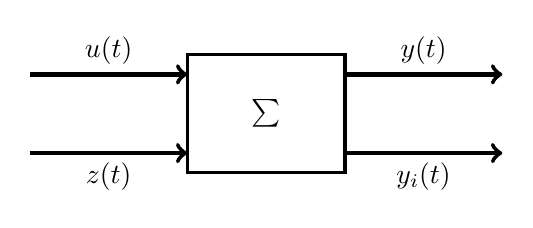
\begin{tikzpicture}[scale=2]

    \node[rectangle, draw, very thick, 
    minimum width = 2cm, 
    minimum height = 1.5cm] (r) at (0,0){\huge $\sum$};

    \draw[->,ultra thick](-1.5,0.25)--(-0.5,0.25);
    \node[above]at(-1,0.25){$u(t)$};

    \draw[->,ultra thick](-1.5,-0.25)--(-0.5,-0.25);
    \node[below]at(-1,-0.25){$z(t)$};

    \draw[->,ultra thick](0.5,0.25)--(1.5,0.25);
    \node[above]at(1,0.25){$y(t)$};

    \draw[->,ultra thick](0.5,-0.25)--(1.5,-0.25);
    \node[below]at(1,-0.25){$y_i(t)$};

\end{tikzpicture}
\end{document}